\section{Bias-Varinace tradeoff}
\begin{figure}[!h]
    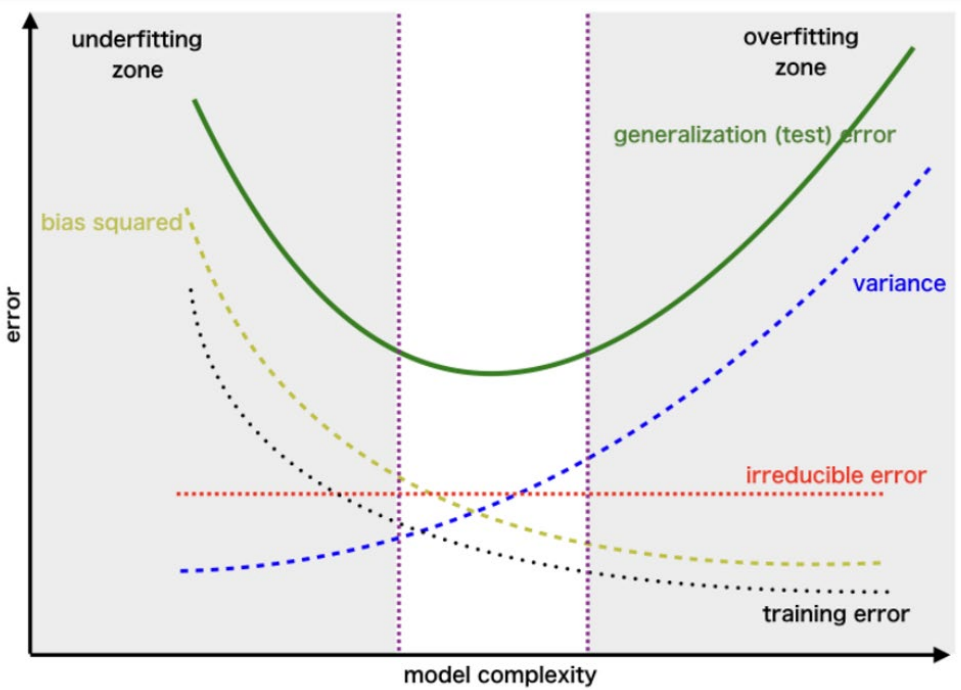
\includegraphics[width = \columnwidth]{figures/03/BiasVariance.png}
\end{figure}
\subsection{No free lunch Theorem}
There is no universally best learner (across problems):

\subsection{Ockham's Razor}
Given 2 models with the same empirical (test) error, the simpler one should be preferred because simplicity is desirable in itself.
\subsection{Error sources and bias-variance tradeoff}
Different Error sources:
\begin{itemize}
    \item The model: the best hypothesis is at distance to the true function
    \item The dataset: different datasets potentially provide different information
    \item Uncertainty in (X,Y) and its representation:
    \subitem Partial view of the task: have all relevant features been observed?
    \subitem Noisy data
\end{itemize}

Error Decomposit MSE:
\[
E_{MSE} = bias + variance + Irreducible \,error
\]
Bias(systematic error): average predictions deviation from the truth

Variance(dependence on specific sample): Sensitivity of prediction to specific training sample

Irreducible error(random nature of process): due to noise

Generally, for more complex/capable model: bias \(\downarrow\),variance \(\uparrow\). Its a trade-off: Only way to redue both is to increase the size of the dataset.

\subsection{Model selection: Validation score and CV score}
\begin{figure}
    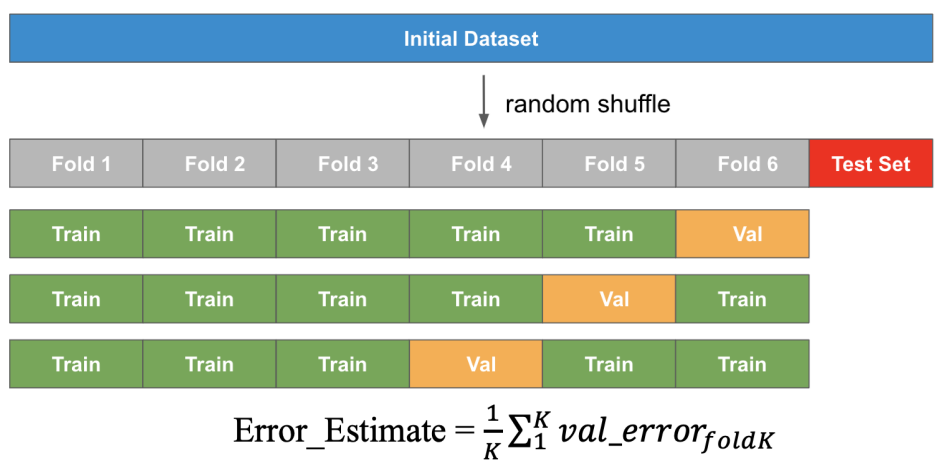
\includegraphics[width = \columnwidth]{figures/03/CV.png}
\end{figure}
k-Fold Corss Validation(CV): We can get a more realistic estimate of the test error using many validation sets (Typically K is 5 to 10)

\subsubsection{Error Estimate Summary}
In practice:
\begin{itemize}
    \item Validation score(s) or CV score provide estimates of the test error
    \item The test error provides an estimate of the true error
    \item Never use any test data in the model training and model selection process
\end{itemize}
Which model to choose?
\begin{itemize}
    \item The one with best validation or CV score
    \item Use student's t-test to check that an improvement is significant
    \item Ockham's razor: prefer simpler models in abscence of other evidence
\end{itemize}
Model selection is an empirical science.
\subsection{Loss minimization (gradient descent)}
Linear Model: \(f(x) = w_0 + w_1 x = \hat{y}\)
\[
RSS = \sum_{i = 1}^{N} (y_i - \hat{y_i})^2
\]
Use gradient of RSS to find optimal weights for model.
\[
\mathbf{w}_{new} = \mathbf{w}_{old}- stepsize \cdot \frac{df(\mathbf{w})}{d\mathbf{w}}
\]
The effectiveness of gradient descent depends on the choice of the learning rate (step size):
\begin{itemize}
    \item Too big, might not reach optimal value
    \item Too small, it will take a long time to converge
\end{itemize}
\subsection{Regularization}
\begin{figure}[!h]
    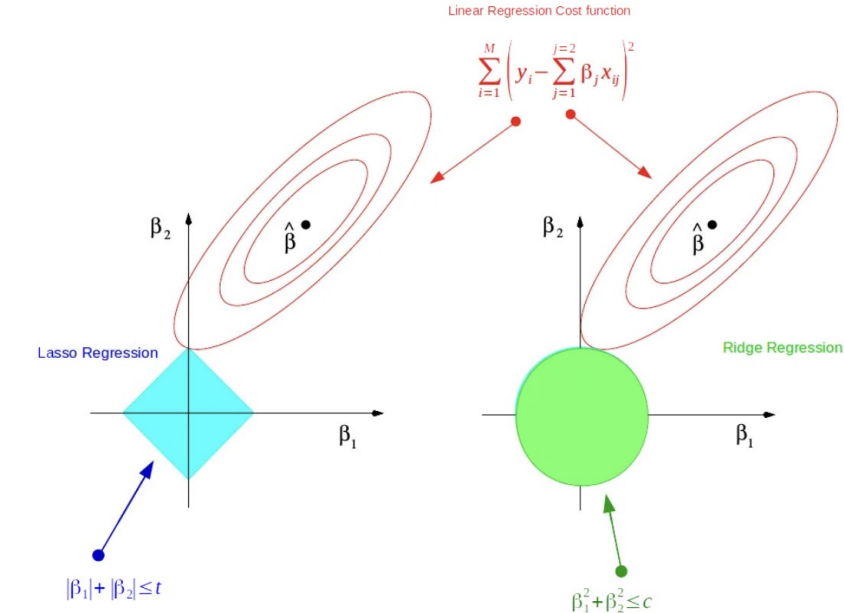
\includegraphics[width = \columnwidth]{figures/03/Regression.png}
\end{figure}

Reduce overfitting of model by penalizing model complexity

Tradeoff:
\begin{itemize}
    \item increase bias
    \item decrease variance
\end{itemize}
\[
H^* = \arg\min_{H \in \mathcal{H}}\sum_{i = 1}^{n}\mathcal{L}_\theta(x_i,y_i) + \lambda R(H)
\]
\(R(H)\) is the models complexity.
\(\lambda\) controlls the model complexity.
\begin{itemize}
    \item Lasso:\(\text{L}_1\) regularization
    \[
    \arg\min\underbrace{||y-X\beta||_2^2}_{\text{Loss}} + \lambda\underbrace{||\beta||_2^2}_{\text{Penalty}}
    \]
    \item Ridge:\(\text{L}_2\) regularization
    \[
    \arg\min\underbrace{||y-X\beta||_2^2}_{\text{Loss}} + \lambda\underbrace{||\beta||_1}_{\text{Penalty}}
    \]
\end{itemize}

\subsection{Hyperparameter tuning}
\begin{figure}[!h]
    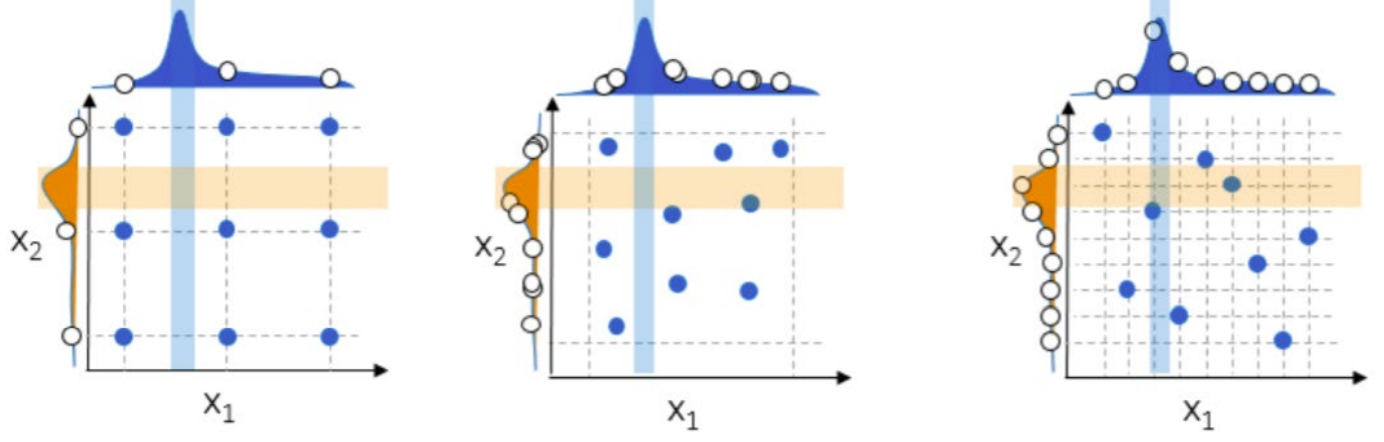
\includegraphics[width = \columnwidth]{figures/03/Hyperparameter.png}
\end{figure}
\begin{itemize}
    \item Grid-search
    \item Random-search
    \item \{Optimization\}
\end{itemize}